\documentclass[10pt, a4paper]{article}

%%% SST LAB PROTOCOLL PREAMBLE
%%% 2019
%%%%%%%%%%%%%%%%%%%%%%%%%%%%%%%


%%% PACKAGES
%%%%%%%%%%%%%%%%%%%%%%%%%%%

\usepackage[ngerman]{babel}

\usepackage[utf8]{inputenc}
\usepackage{amsmath}
\usepackage{pgfplots}
\usepackage{tikz}
\usepackage[many]{tcolorbox}
\usepackage{graphicx}
\graphicspath{ {./graphics/} }
\usepackage{pdfpages}
\usepackage{dashrule}
\usepackage{float}
\usepackage{siunitx}
\usepackage{trfsigns}
\usepackage{booktabs}
\usepackage[european]{circuitikz}
\usepackage{tcolorbox}

%%% DOCUMENT GEOMETRY
%%%%%%%%%%%%%%%%%%%%%%%%%%%

\usepackage{geometry}
\geometry{
 a4paper,
 total={0.6180339887498948\paperwidth,0.6180339887498948\paperheight},
 top = 0.1458980337503154\paperheight,
 bottom = 0.1458980337503154\paperheight
 }
\setlength{\jot}{0.013155617496424828\paperheight}
\linespread{1.1458980337503154}

\setlength{\parskip}{0.013155617496424828\paperheight} % paragraph spacing


%%% COLORS
%%%%%%%%%%%%%%%%%%%%%%%%%%%

\definecolor{red1}{HTML}{f38181}
\definecolor{yellow1}{HTML}{fce38a}
\definecolor{green1}{HTML}{95e1d3}
\definecolor{blue1}{HTML}{66bfbf}
\definecolor{hsblue}{HTML}{00b1db}
\definecolor{hsgrey}{HTML}{afafaf}

%%% CONSTANTS
%%%%%%%%%%%%%%%%%%%%%%%%%%%
\newlength{\smallvert}
\setlength{\smallvert}{0.0131556\paperheight}


%%% COMMANDS
%%%%%%%%%%%%%%%%%%%%%%%%%%%

% differential d
\newcommand*\dif{\mathop{}\!\mathrm{d}}

% horizontal line
\newcommand{\holine}[1]{
  	\begin{center}
	  	\noindent{\color{hsgrey}\hdashrule[0ex]{#1}{1pt}{3mm}}\\%[0.0131556\paperheight]
  	\end{center}
}

% mini section
\newcommand{\minisec}[1]{ \noindent\underline{\textit {#1} } \\}

% quick function plot
\newcommand{\plotfun}[3]{
  \vspace{0.021286\paperheight}
  \begin{center}
    \begin{tikzpicture}
      \begin{axis}[
        axis x line=center,
        axis y line=center,
        ]
        \addplot[draw=red1][domain=#2:#3]{#1};
      \end{axis}
    \end{tikzpicture}
  \end{center}
}

% box for notes
\newcommand{\notebox}[1]{

\tcbset{colback=white,colframe=green1!100!black,title=Note!,width=0.618\paperwidth,arc=0pt}

 \begin{center}
  \begin{tcolorbox}[]
   #1 
  \end{tcolorbox}
 
 \end{center} 
 
}

% box for equation
\newcommand{\eqbox}[2]{
	
	\tcbset{colback=white,colframe=green1!100!black,title=,width=#2,arc=0pt}
	
	\begin{center}
		\begin{tcolorbox}[ams align*]
				#1
		\end{tcolorbox}
		
	\end{center} 
	
}
% END OF PREAMBLE

\renewcommand{\familydefault}{\sfdefault}

\addbibresource{sources.bib}

\begin{document}


\includepdf{./titlepage/titlepage.pdf}
\pagebreak

\newpage
  \tableofcontents
\newpage

\section{Einführung}
Network Intrusion Detection Systems (NIDS) sind Anwendungen, die versuchen, schädliche Aktivitäten im Netzwerk zu erkennen, indem sie dessen gesamten Traffic aufzeichnen und analysieren. Ein beliebtes NIDS-Programm ist das free/open-source tool \textbf{snort}, welches hier zum Einsatz kommt. Es bietet ein modulares Konfigurationssystem über sog. \textit{rules} für Traffic- und Protokollanalysen sowie die Erkennung verschiedenster Angriffe über Signaturmatching.\\

Dieses Dokument beschreibt die Installation einer Testumgebung für snort auf Basis von VirtualBox, welche anschließend durch verschiedene Angriffe getestet wird. Die Netzwerkstruktur zeigt die folgende Abb. \ref{fig:network-structure}.

\begin{figure}[H]
  \centering
  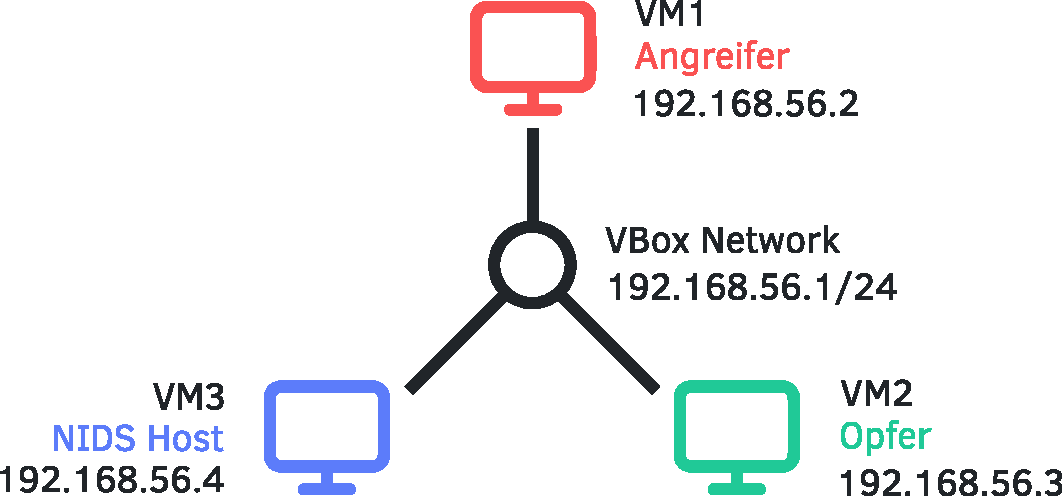
\includegraphics[width=0.6\textwidth]{graphics/intro/network.pdf}
  \caption{Virtuelle Netzwerkstruktur.}\label{fig:network-structure}
\end{figure}

Die drei virtuellen Maschinen befinden sich im gleichen virtuellen Netzwerk. Ein Angreifersystem (Kali Linux) versucht, Hosts im Netzwerk mit unterschiedlichen Methoden anzugreifen. Der NIDS-Host sollte dann mit snort diese Aktivitäten erkennen.\\

Zunächst folgt das Setup der Testumgebung.


\section{Setup}
\subsection{Installation der Virtuellen Maschinen}
Die drei virtuellen Maschinen werden unter Oracle VirtualBox entsprechend Tabelle \ref{tab:host-config} installiert. Die Installationen erfolgen mit den jeweiligen grafischen Installern, wobei grundsätzlich die Standardeinstellungen verwendet werden. Für die beiden Debian-Systeme wure keine Desktopoberfläche ausgewählt (lediglich \inlinecodee{standard system utilities}). Abb. \ref{fig:vbox-group} zeigt die virtuellen Maschinen unter Virtualbox.

\begin{figure}[h]
  \centering
  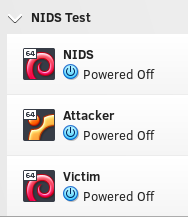
\includegraphics[width=0.2\textwidth]{graphics/setup/vbox_group.png}
  \caption{Verwendete Maschinen in Virtualbox.}\label{fig:vbox-group}
\end{figure}

\subsection{Snort-Installation}

Als nächstes wird snort auf der NIDS-VM installiert.
\begin{minted}{bash}
  su
  apt install snort
\end{minted}

Bei der Installation erscheint ein Konfigurationsfenster. In dieses muss die CIDR-Adresse des VirtualBox-Netzwerkes (\inlinecodee{192.168.56.0/24}) eingetragen werden (Abb. \ref{fig:snort-first-time-setup}).

\begin{figure}[H]
  \centering
  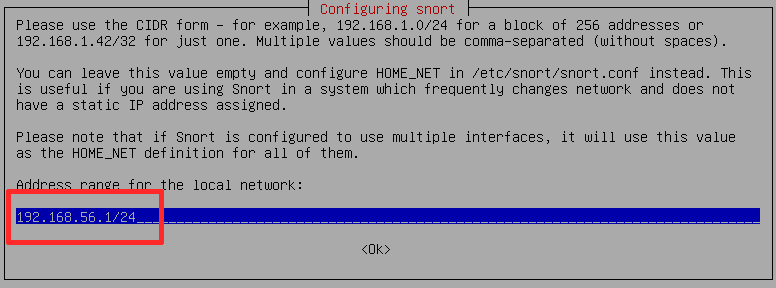
\includegraphics[width=0.5\textwidth]{graphics/setup/config-snort-1.png}
  \caption{Snort Konfiguration bei der Installation.}\label{fig:snort-first-time-setup}
\end{figure}

Mit dem folgenden Befehl kann die snort-Installation überprüft werden.
\begin{minted}{bash}
  /sbin/snort --version
\end{minted}

\subsection{Webserver-Installation}
\inlinecodee{nginx} wird auf dem Victim-Host als Ziel für den Angreifer installiert. Dazu wird lediglich folgender Befehl ausgeführt.
\begin{minted}{bash}
  su
  apt install nginx
\end{minted}

\subsection{Erstellen des Virtuellen Netzwerkes}
Um das virtuelle Netzwerk einzurichten, öffnet man zunächst \inlinecodee{File -> Tools -> Network Manager} und erstellt ein neues Netzwerk mit der Schaltfläche \inlinecodee{Create} (Abb. \ref{fig:network-host-manager}).

\begin{figure}[H]
  \centering
  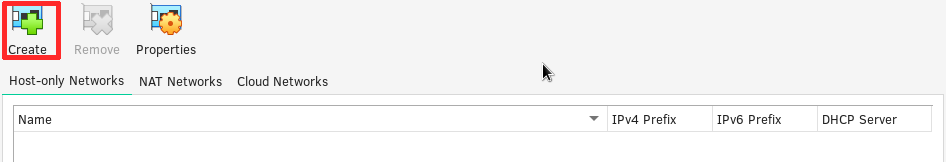
\includegraphics[width=0.8\textwidth]{graphics/setup/network-create.png}
  \caption{Erstellen des virtuellen Netzwerkadapters}\label{fig:network-host-manager}
\end{figure}

Danach kann man über \inlinecodee{Properties} die in Abb. \ref{fig:network-hm-properties} zu sehenden Einstellungen eintragen.

\begin{figure}[H]
  \centering
  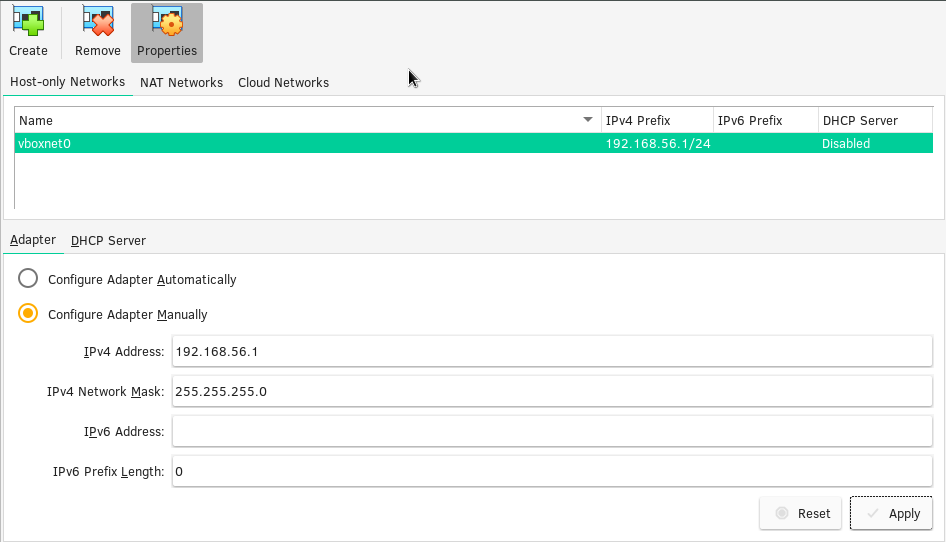
\includegraphics[width=0.8\textwidth]{graphics/setup/network-adapter.png}
  \caption{Einstellungen des Netzwerkadapters}\label{fig:network-hm-properties}
\end{figure}

Um die drei Hosts mit dem neuen virtuellen Adapter zu verbinden, wählt man die jeweilige Maschine aus, öffnet \inlinecodee{Settings} und wechselt zum \inlinecodee{Network}-Tab. Danach wählt man \inlinecodee{Adapter 2}, aktiviert ihn, setzt \inlinecodee{Attached to:} auf \inlinecodee{Host-only Adapter} und wählt den vorher erstellten Adapter aus (Abb. \ref{network-host-setup1}, \ref{network-host-setup2})

\begin{figure}[H]
  \begin{minipage}[t]{0.45\textwidth}
    \centering
    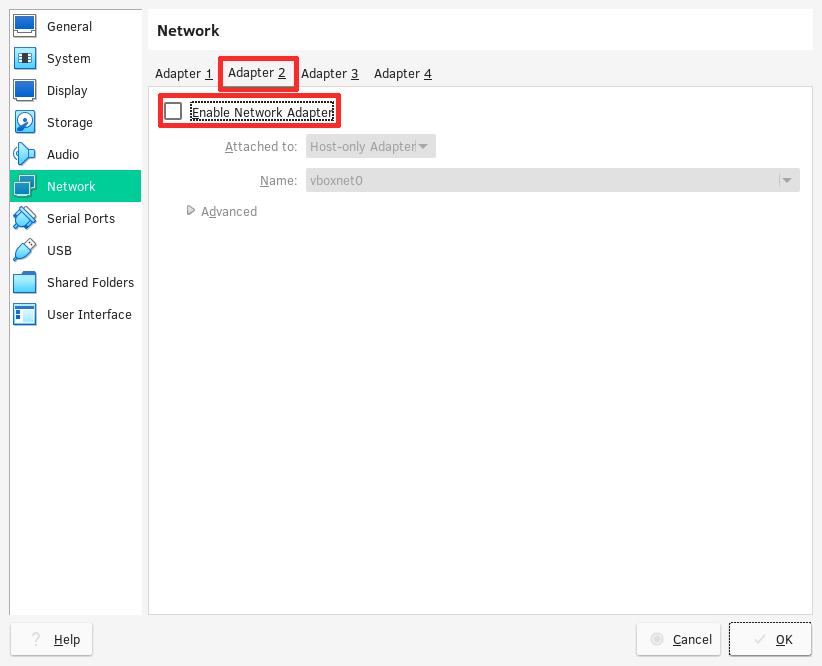
\includegraphics[width=\textwidth]{graphics/setup/network-host-setup1.png}
    \caption{Aktivieren von Adapter 2.}\label{network-host-setup1}
  \end{minipage}\hfill
  \begin{minipage}[t]{0.45\textwidth}
    \centering
    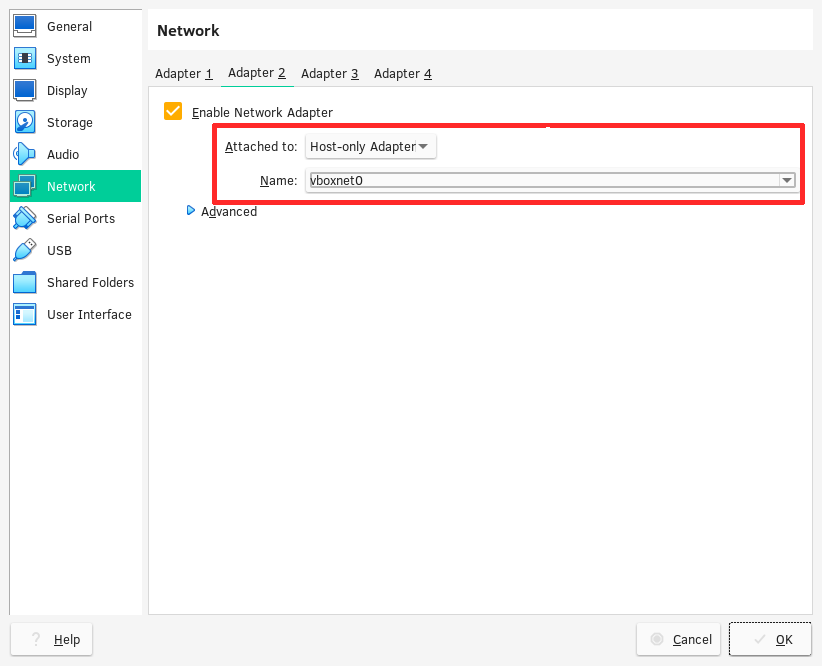
\includegraphics[width=\textwidth]{graphics/setup/network-host-setup2.png}
    \caption{Auswählen des Adapters.}\label{network-host-setup2}
   \end{minipage}
\end{figure}

Damit snort den Netzwerktraffic anderer Hosts sniffen kann, muss zuletzt für die NIDS-Maschine der Promiscuous-Modus aktiviert werden (Abb. \ref{fig:promisc}).

\begin{figure}[H]
  \centering
  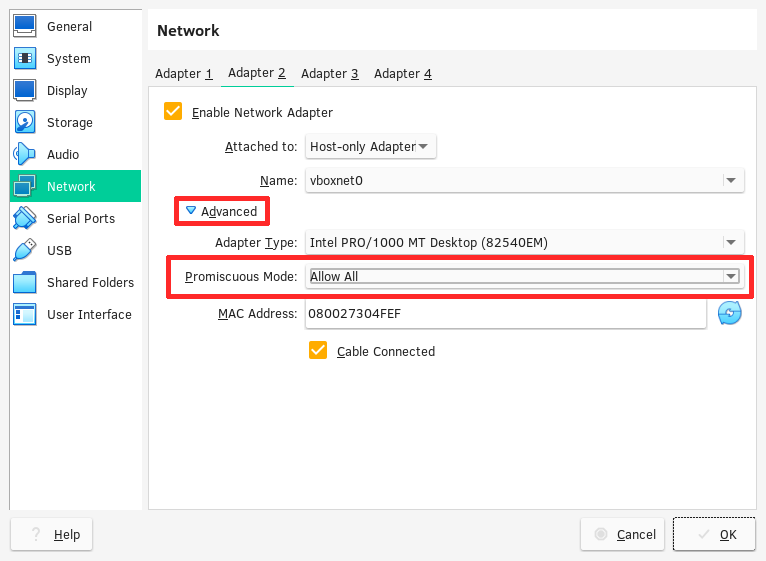
\includegraphics[width=0.5\textwidth]{graphics/setup/promisc.png}
  \caption{Promiscuous Mode für den NIDS-Host.}\label{fig:promisc}
\end{figure}


\subsection{IP-Adressen-Vergabe}\label{sec:ip-dist}
Jeder Host erhält eine statische IP-Adresse aus Reproduzierbarkeitsgründen. Diese können Tabelle \ref{tab:host-config} entnommen werden. Hierzu muss zuerst die Adapterbezeichnung auf der jeweiligen Maschine herausgefunden werden. Dies gelingt mit dem Befehl \inlinecodee{ip addr show} (Abb. \ref{fig:ip-addr-show})

\begin{figure}[H]
  \centering
  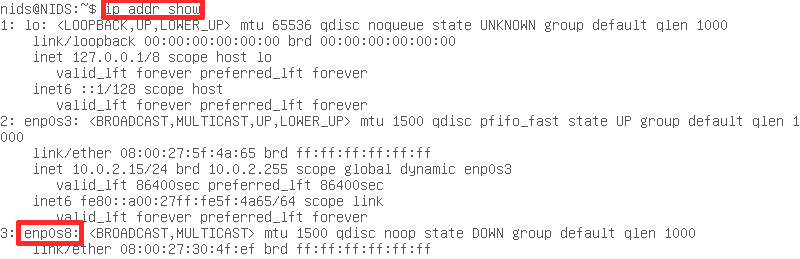
\includegraphics[width=0.8\textwidth]{graphics/setup/static-ip-1.png}
  \caption{VM-Netzwerkinterfaces.}\label{fig:ip-addr-show}
\end{figure}

Danach muss die Datei \inlinecodee{/etc/network/interfaces} entsprechend Abb. \ref{fig:static-ip-1} bearbeitet werden und der \inlinecodee{networking} Service neugestartet werden.

\begin{figure}[H]
  \centering
  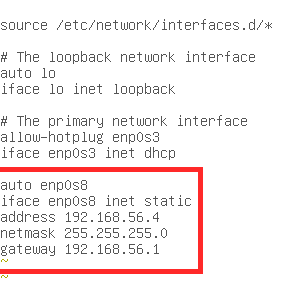
\includegraphics[width=0.25\textwidth]{graphics/setup/static-ip-2.png}
  \caption{\inlinecodee{/etc/network/interfaces}.}\label{fig:static-ip-1}
\end{figure}


\begin{minted}{bash}
    $ sudo systemctl restart networking.service
\end{minted}

Wurde dies für alle VMs durchgeführt, kann ein einfacher Verbindungstest über den \inlinecodee{ping}-Befehl ausgeführt werden.

\begin{table}
  \centering
\begin{tabular}{|l|l|l|l|l|l|}
\hline
ID  & OS & Hostname & user & password & IP \\ \hline
VM1 & Kali Linux & Attacker & attacker & 0000 &  192.168.56.2 \\ \hline
VM2 & Debian & Victim & victim & 0000 & 192.168.56.3 \\ \hline
VM3 & Debian & NIDS & nids & 0000 &192.168.56.4 \\
\hline
\end{tabular}
\caption{Zusammenfassung der Host-Konfigurationen}\label{tab:host-config}
\end{table}



\section{NIDS-Konfiguration und Angriffe}

\subsection{Snort-Konfiguration}

Die Hauptkonfigurationsdatei für snort liegt unter \inlinecodee{/etc/snort/snort.conf}. In diesem Fall muss allerdings zuerst die Debian-spezifische Datei \inlinecodee{/etc/snort/snort.debian.conf} entsprechend Abb. \ref{fig:snort-debian-conf} bearbeitet werden. Das Feld \inlinecodee{DEBIAN\_SNORT\_INTERFACE} wird entsprechend Abschnitt \ref{sec:ip-dist} gesetzt.

\begin{figure}[H]
\centering
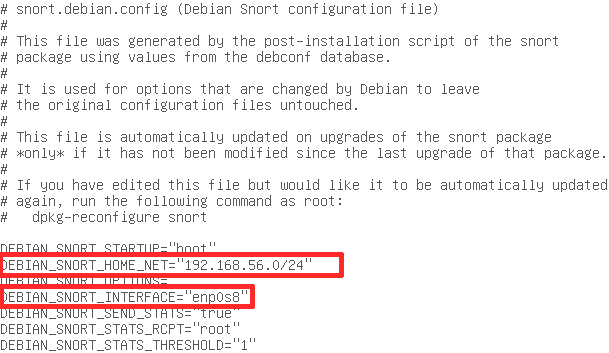
\includegraphics[width=0.6\textwidth]{graphics/attacks/snort-debian.png}
\caption{\inlinecodee{/etc/snort/snort.debian.conf}}\label{fig:snort-debian-conf}
\end{figure}


Es gibt einige vorgefertigte Regeln, welche unter \inlinecodee{/etc/snort/rules} zu finden sind.
In \inlinecodee{/etc/snort/snort.conf} findet man am Ende der Datei alle Regeln (Pfade), die snort einbeziehen soll, d.h die Regeln, die tatsächlich aktiv sind.

Um die Konfiguration nach dem Bearbeiten auf Fehler zu prüfen, kann man folgenden Befehl nutzen.
\begin{minted}{bash}
  /sbin/snort -T -i enp0s8 -c /etc/snort/snort.conf
\end{minted}

\notebo{Info}{
Snort kann über die Tastenkombinaition \inlinecodee{Ctrl+z} beendet werden.
}


\subsection{Benutzerdefinierte Regeln}

Die Regeldefinitionen folgen einer einfachen Syntax. Die grundlegende Struktur zeigt Abb. \ref{fig:snort-rule-syntax}. Als Referenz eignen sich auch die vorgefertigten Regeln unter \inlinecodee{/etc/snort/rules}.

\begin{figure}[H]
\centering
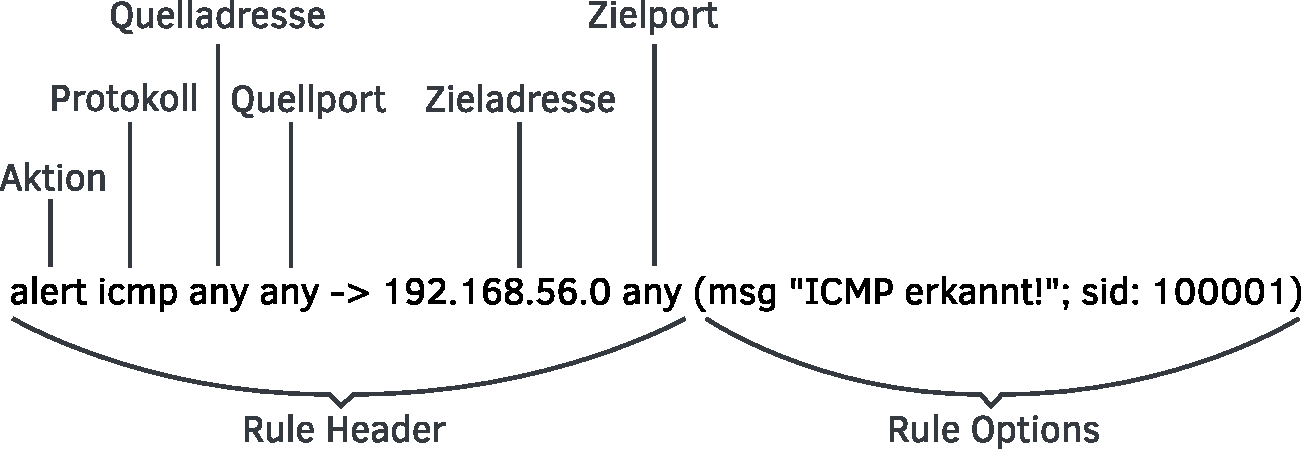
\includegraphics[width=0.6\textwidth]{graphics/attacks/rule-syntax.pdf}
\caption{Struktur der Snort-Regeln.}\label{fig:snort-rule-syntax}
\end{figure}

Die dargestellte Regel alarmiert bei Erkennung eines ICMP-Paketes (z.B. ping). Um sie hinzuzufügen fügt man die Zeile aus Abb \ref{fig:snort-rule-syntax} in die zuerst leere Datei \inlinecodee{/etc/snort/rules/local.rules} ein. Die Zieladresse kann auch durch die Umgebungsvariable \inlinecodee{\$HOME\_{NET}} ersetzt werden (Abb. \ref{fig:snort-localrules1}). \footnote{Die \inlinecodee{sid} kann quasi ein beliebiger einzigartiger Wert sein.}\\

\begin{figure}[H]
\centering
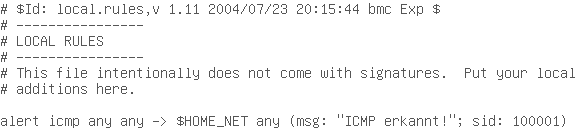
\includegraphics[width=0.6\textwidth]{graphics/attacks/localrules1.png}
\caption{\inlinecodee{/etc/snort/rules/local.rules}}\label{fig:snort-localrules1}
\end{figure}


Dann startet man snort mit dem Befehl
\begin{minted}{bash}
  /sbin/snort -q -l /var/log/snort -i enp0s8 -A console -c /etc/snort/snort.conf
\end{minted}

Danach kann vom Angreifer ein \inlinecodee{ping}-Befehl auf den Victim-Host durchgeführt werden, welcher wie in Abb. \ref{fig:snort-ping} durch snort erkannt werden sollte.

\begin{figure}[H]
  \centering
  
\includegraphics[width=0.8\textwidth]{graphics/attacks/snort-ping.png}
  \caption{Ergebnis des Ping-Tests.}\label{fig:snort-ping}
\end{figure}

Als Hilfe zur Erstellung von Regeln eignet sich die Website \textit{snorpy} \cite{snorpy}, welche eine grafische Oberfläche bietet, um Regeln zu erstellen und mögliche Optionen zu erkunden.

\subsection{nmap}
Mit der Standardkonfiguration lässt sich ein einfacher \inlinecodee{nmap}-Scan sofort erkennen.\\
Vom Angreifer aus:
\begin{minted}{bash}
  nmap 192.168.56.3
\end{minted}

\begin{figure}[H]
  \centering
  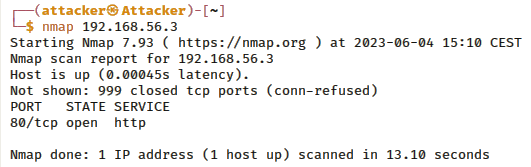
\includegraphics[width=0.5\textwidth]{graphics/attacks/nmap-kali-working.png}
  \caption{Ergebnis von nmap beim Angreifer.}\label{fig:nmap2}
\end{figure}

Das Resultat des NIDS zeigt Abb. \ref{fig:nmap1}.

\begin{figure}[H]
  \centering
  
\includegraphics[width=0.8\textwidth]{graphics/attacks/nmap.png}
  \caption{NIDS altert bei nmap.}\label{fig:nmap1}
\end{figure}

\subsection{DoS-Angriff / SYN-Flood}\label{sec:dos}

Die Standardkonfiguration von snort kann bereits DoS-Angriffe erkennen. Für eine einfache benutzerdefinierte Konfiguration kann man die folgende Regel verwenden.

\begin{minted}{bash}
  alert tcp any -> $HOME_NET 80 (flag: S; msg: "Potentieller DoS-Angriff!"; sid: 100002)
\end{minted}

Hierbei wird die Option \inlinecodee{flag: S} genutzt, um TCP-Pakete zu erkennen, bei denen nur das SYN-Flag gesetzt ist. Weitere Flags finden sich in der snort-Dokumentation \cite{snortflag}.\\

Der Webserver auf dem Victim-Host sollte bereits mit einer Beispielseite laufen. Dies kann z.B. über Firefox auf dem Angreifer überprüft werden. Da der Webbrowser aufgrund von Caching ungeeignet ist für die Erkennung des Serverzustandes, kann man alternativ den folgenden Befehl nutzen.

\begin{minted}{bash}
  curl -I 192.168.56.3
\end{minted}

Dieser sollte bei erfolgreicher Bearbeitung durch den Server die in Abb. \ref{fig:nginx-1} zu sehende Ausgabe liefern.\\

\begin{figure}[H]
\centering
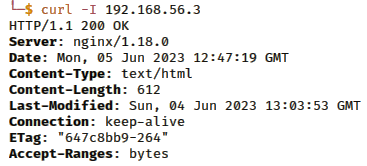
\includegraphics[width=0.4\textwidth]{graphics/attacks/curl-result1.png}
\caption{Erfolgreiche Webserverantwort.}\label{fig:nginx-1}
\end{figure}

Das auf Kali vorinstallierte Tool \inlinecodee{hping3} kann nun für einen einfachen TCP SYN-Angriff verwendet werden. Dazu wird folgender Befehl genutzt.\\

\begin{minted}{bash}
  sudo hping3 --flood -S --rand-source -p 80 192.168.56.3
\end{minted}

Nun kann die Seite erneut angefragt werden (z.B. auf dem Angreifer-System). Es sollte zu Verzögerungen kommen. Gleichzeitig sollte das snort-System die Anfragen als \glqq{}Potentially Bad Traffic\grqq{} klassifizieren (Abb. \ref{fig:dos-snort}). Als Variation kann man das Argument \inlinecodee{--rand-source} im \inlinecodee{hping3} weglassen.
Sind keine Verzögerungen merkbar, kann der folgende alternative Befehl zu Anfrage möglicherweise helfen.
\begin{minted}{bash}
  curl -I 192.168.56.3 -H "Cache-Control: no cache"
\end{minted}

\begin{figure}[H]
\centering
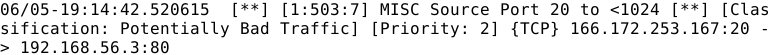
\includegraphics[width=0.6\textwidth]{graphics/attacks/snort-dos.png}
\caption{SYN-Angriffserkennung durch snort.}\label{fig:dos-snort}
\end{figure}


\section{Wireshark}
Die mit dem snort-Flag \inlinecodee{l} generierten Logdateien enthalten nicht die Alarmierungsnachrichten der Konsole, sondern sind Logs des gesamten Traffics. Praktischerweise können diese mit Wireshark geöffnet und nachträglich analysiert werden. Mithilfe der Konsolenausgabe oder eines externen Logs (über Option \inlinecodee{-A fast}) können dann z.B. die Zeiten der Alarme genutzt werden, um die Angriffe in Wireshark ausfindig zu machen. Abb. \ref{fig:wireshark} zeigt einen Ausschnitt der SYN-Flood aus Abschnitt \ref{sec:dos}.

\begin{figure}[H]
\centering
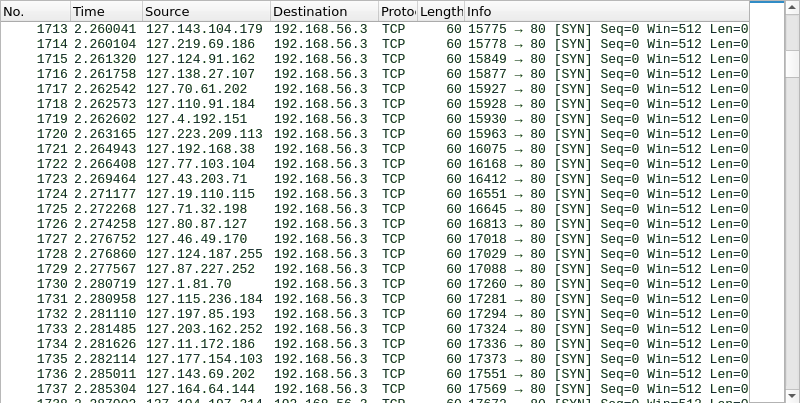
\includegraphics[width=0.7\textwidth]{graphics/attacks/wireshark.png}
\caption{Snort Log in Wireshark}\label{fig:wireshark}
\end{figure}


\section{Zusammenfassung}
Die dargestellten Beispiele bieten einen einfachen Einstieg in snort und die Funktionsweise von dessen Regeln. Komplexere Beispiele mit gezielten Attacken auf Vulnerabilitäten (z.B. MS EternalBlue) und deren Erkennung durch das NIDS könnten in einer fortführenden Arbeit behandelt werden.


\begin{refsection}[sources.bib]
\nocite{*}
\printbibliography[heading=subbibliography,title={Referenzen}]
\end{refsection}


\end{document}
